\documentclass[a5paper,titlepage,10pt,openany]{scrbook}
\usepackage[a5paper,backref]{hyperref}
\usepackage[papersize={148.5mm,215mm},twoside,bindingoffset=0.5cm,hmargin={2cm,2cm},
				vmargin={2cm,2cm},footskip=1.1cm,driver=dvipdfm]{geometry}
\usepackage{palatino}
\usepackage{pstricks}
\usepackage{graphicx}
\usepackage{floatflt}
\usepackage[bahasa]{babel} 
%\usepackage[pdftex]{dropping}
\usepackage{lettrine}
\author{Lingkungan St. Petrus Maguwo}
\title{Warta Iman}
\setlength{\parindent}{1cm}
\psset{unit=1mm}

\makeatletter
\renewcommand{\@makeschapterhead}[1]{%
  {\parindent \z@ \centering \normalfont
    \interlinepenalty\@M \Large \bfseries #1\par\nobreak \vskip 20\p@ }}
\renewcommand{\section}{\@startsection {section}{1}{\z@}%
                                   {-3.5ex \@plus -1ex \@minus -.2ex}%
                                   {2.3ex \@plus.2ex}%
%                                   {\normalfont\normalsize\bfseries\centering}}
                                   {\normalfont\normalsize\bfseries}}
\renewcommand\subsection{\@startsection{subsection}{2}{\z@}%
                                     {-3.25ex\@plus -1ex \@minus -.2ex}%
                                     {1.5ex \@plus .2ex}%
                                     {\normalfont\normalsize\bfseries}}
\renewcommand\subsubsection{\@startsection{subsubsection}{3}{\parindent}%
                                    {3.25ex \@plus1ex \@minus.2ex}%
                                    {-1em}%
                                    {\normalfont\normalsize\bfseries}}
\makeatother
\hyphenation{sa-u-da-ra-ku}
\hyphenation{ke-ri-ngat}
\hyphenation{je-ri-tan}
\hyphenation{hu-bung-an}
\hyphenation{me-nya-dari}
\hyphenation{Eng-kau}
\hyphenation{ke-sa-lah-an}
\hyphenation{ba-gai-ma-na}
\hyphenation{Tu-han}
\hyphenation{di-per-ca-ya-kan}
\hyphenation{men-ja-uh-kan}
\hyphenation{bu-kan-lah}
\hyphenation{per-sa-tu-kan-lah}
\hyphenation{ma-khluk}
\hyphenation{Sem-buh-kan-lah}
\hyphenation{ja-lan}
\hyphenation{mem-bu-tuh-kan}
\hyphenation{be-ri-kan-lah}
\hyphenation{me-ra-sa-kan}
\hyphenation{te-man-ilah}
\hyphenation{mem-bi-ngung-kan}
\hyphenation{di-ka-gum-i}
\hyphenation{ta-ngis-an-Mu}
\hyphenation{mi-lik-ilah}


\begin{document}
\thispagestyle{empty}
\newcommand{\edisi}[1]{%
\DeclareFixedFont{\PT}{T1}{ppl}{b}{}{0.7in}
\DeclareFixedFont{\PTit}{T1}{ppl}{b}{it}{0.7in}
\DeclareFixedFont{\PTsmall}{T1}{ppl}{b}{it}{0.25in}
\DeclareFixedFont{\PTsmaller}{T1}{ppl}{b}{it}{0.175in}
\DeclareFixedFont{\PTsmallest}{T1}{ppl}{b}{it}{0.15in}

\begin{pspicture}(14cm,2cm)
\rput[rb](10.35cm,3cm){\PTsmallest {#1}}
\rput[lb](-2cm,1.5cm){\PT {WARTA IMAN}}
\rput[lb](0cm,0.5cm){\PTsmall {Lingkungan St. Petrus Maguwo}}
\end{pspicture}%
}

\newcounter{kgkcounter}[chapter]
\renewcommand{\thekgkcounter}{\arabic{kgkcounter}. }
\newcommand{\kgk}[1]{\refstepcounter{kgkcounter}\textbf{\flushleft \textbf{\thekgkcounter #1}}\\}

\newcommand{\kutipan}[1]{%
\noindent{\framebox{\parbox{10cm}{\centering\emph{#1}}}}}

\edisi{November 2011}

%\vspace{1cm}

\begin{center}
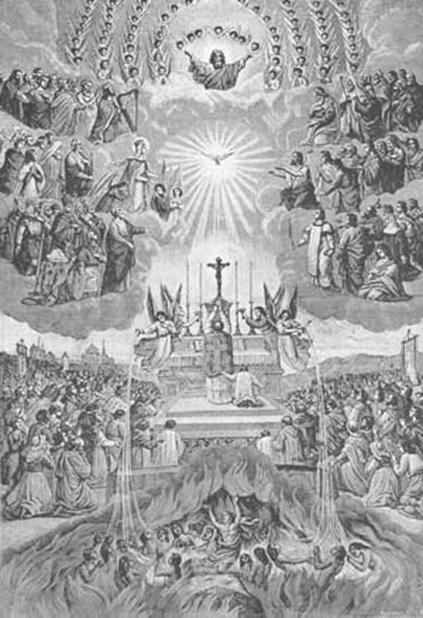
\includegraphics[scale=0.85]{gambar/purgatory2.jpg}
\end{center}

%\vspace{1cm}

\begin{center}
{\PTsmaller {Kasih, kerendahan hati, dan menurut pada kehendak Allah }}
\end{center}

\newpage

\chapter*{Dari Redaksi}
\footnotesize
\indent{Berkah Dalem,}
Bulan Maret sudah memasuki masa Prapaskah. Tidak ada salahnya jika kita mengambil tema \textit{Prapaskah} untuk edisi kali ini. Mungkin kita masih bertanya-tanya kenapa setiap masa prapaskah kita berpuasa dan berpantang. Bagian awal WI edisi kali mencoba menjawab pertanyaan tersebut.

\bigskip
Menjelang prapaskah kita sudah mendengar pembacaan pesan Bapa Uskup dalam menyongsong masa prapaskah. Dalam edisi ini Anda dapat menyimak pesan dari Bapa Paus Benediktus dalam rangka menyongsong Prapaskah 2012.

\bigskip
Masa prapaskah diawali dengan hari Rabu Abu. Kenapa Rabu dan kenapa abu? Juga kenapa digunakan daun palm bukan yang lain? Jawabannya dapat Anda simak dalam edisi kali ini. 
 
\bigskip
Renungan tentang 4 prinsip hidup dan ketika garam kehilangan asinnya melengkapi edisi kali ini. Kutipan Kompendium Gereja Katolik masih berlanjut sampai pada nomor 30 -- 33.

\bigskip

Warta lingkungan kali ini tidak memuat pasangan yang berulangtahun, karena data yang ada redaksi tidak ditemukan warga St. Petrus yang berulangtahun perkawinan bulan Maret. Redaksi tetap berharap partisipasi umat untuk meramaikan rubrik ini dengan mengirim sms berupa saran, kritik, pertanyaan, atau sekedar \textit{uneg-uneg}, dengan harapan terjalin komunikasi antar umat dan juga pengurus. Tema bulan April adalah Paskah sedang bulan Mei adalah Liturgi. Sekali lagi ditunggu partisipasi seluruh umat.
\normalsize

\begin{center}***\end{center} 

\vfill

\noindent{\framebox{\parbox{10cm}{\small
Warta Iman\\
Media komunikasi dan informasi umat lingkungan St. Petrus\\
Alamat Redaksi: Lingkungan St. Petrus Maguwo\\
E-mail: stpetrusmgw@gmail.com
}}}
\normalsize


\chapter*{\begin{center}Bagaimana Kita Menghormati Bunda Maria\end{center}}			
\begin{center}\textit{Tim Carmelia}\end{center}	   

\subsection*{PENGANTAR}
Sebagai orang Katolik, kita harus mengenal bagaimana peranaan Bunda Maria dalam Gereja, karena Maria adalah Bunda Gereja. Kita tidak dapat melihat kedudukan Bunda Maria dengan perasaan kita, tetapi kita harus mengacu kepada tafsiran Gereja dan tafsiran Kitab Suci. Orang Katolik menghormati Bunda Maria, fakta ini menimbulkan pertanyaan bagi sebagian orang, batu sandungan, kadang-kadang menjadi bahan tuduhan dari saudara-saudari kita yang berkepercayaan lain. Dari kritikan ini mengakibatkan begitu banyak orang Katolik yang tidak tertarik lagi untuk menghormati Bunda Maria bahkan meninggalkan Gereja Katolik.
Tuduhan-tuduhan yang sering kita dengar antara lain: orang Katolik menghormati Bunda Maria secara berlebihan, atau orang Katolik menyembah Maria, atau orang Katolik menyembah patung. Menghadapi pertanyaan- pertanyaan seperti ini, kita tidak bisa hanya membiarkannya berlalu begitu saja atau melarikan diri, tetapi kita harus berusaha menjawabnya sambil merenung apakah penghormatan kita kepada Bunda Maria sudah benar atau salah.

\subsection*{SYARAT-SYARAT PENGHORMATAN KEPADA BUNDA MARIA}
Dalam penghormatan kepada Bunda Maria, kita berpedoman pada empat sifat, yaitu:
\begin{enumerate}
\item Penghormatan kepada Bunda Maria harus berdasarkan Kitab Suci.

Dalam Kitab Suci memang tidak ada satu ayat pun yang menyuruh kita untuk menghormati Bunda Maria. Akan tetapi dalam Injil Lukas 1:26-38 dan ayat paralelnya, kita menemukan dasar mengapa kita menghormati Bunda Maria. Dasar-dasar dalam menghormati Bunda Maria antara lain:
\begin{itemize}
\item Bunda Maria terlibat aktif dalam karya penebusan

Seperti dalam dalam Injil Lukas, ketika Malaikat Gabriel menyampaikan pesan Allah kepada Bunda Maria bahwa ia akan melahirkan seorang laki-laki. ”Sesungguhnya engkau akan mengandung dan melahirkan seorang anak laki-laki dan hendaklah engkau menamakan Dia Yesus. Ia akan menjadi besar dan akan disebut Anak Allah yang Mahatinggi. Dan Tuhan Allah akan mengaruniakan kepada-Nya takhta Daud, bapa leluhurnya” (Luk 1:31-32). Bunda Maria dengan iman yang penuh, pasrah kepada Allah dan hanya menjawab: “Sesungguhnya aku ini hamba Tuhan terjadilah padaku menurut perkataanmu” (Luk 1:38). Di sinilah Bunda Maria menerima tugas untuk mengambil bagian dalam karya keselamatan. Seluruh hidup Bunda Maria diabdikan kepada karya penebusan. Apa yang dibuat oleh Bunda Maria? Bunda Maria mengandung dan kemudian melahirkan Sang Penebus, dan sebagai akibatnya ia harus mengungsi ke Mesir. Kemudian Bunda Maria harus membesarkan anaknya itu yaitu Tuhan Yesus, dengan segala kebutuhan-Nya. Dengan demikian Bunda Maria terlibat penuh dalam karya penebusan.
\item Bunda Maria merupakan seorang kudus yang besar

Dalam Gereja katolik kita menghormati orang-orang kudus karena mereka merupakan karya tangan Tuhan yang penuh dan kaya akan rahmat. Bunda Maria adalah yang terkudus dari para kudus Bahkan sejak dalam kandungan Santa Anna, ia sudah dipersiapkan oleh Allah sebagai ibu penyelamat. Maka pantaslah kita menghormatinya sebagai karya tangan Allah yang istimewa. Dikatakan oleh malaikat: “Salam hai engkau yang dikarunia, Tuhan menyertai engkau.” Suci artinya dikaruniai oleh Tuhan. Orang dijadikan suci bukan karena karya manusia, doa manusia, kepandaian, tetapi pertama-tama oleh karena karunia Tuhan. Dari dalam diri manusia dibutuhkan suatu jawaban yang serius akan rahmat Tuhan yang istimewa ini, karena rahmat membutuhkan kerja sama dengan usaha manusia, tetapi yang menjadi penggerak utama adalah rahmat Tuhan. Ketika malaikat mengatakan “salam hai engkau yang dikaruniai Tuhan”, di sinilah malaikat mengakui bahwa Maria adalah orang yang kudus.
\end{itemize}


\item Penghormatan kepada Bunda Maria harus sesuai dengan liturgi/ibadat.

Pusat ibadat/liturgi dalam Gereja Katolik hanyalah satu, yaitu Allah sendiri melalui Putra-Nya, Yesus Kristus. Segala penghormatan kita harus sampai kepada Allah, menghormati Bunda Maria tidak hanya sampai pada Maria itu sendiri, agar tidak mengambil arti atau mengambil kesimpulan singkat bahwa kita menjadikan Bunda Maria sebagai Allah. Kita harus menghormati Bunda Maria supaya ia menghantar kita kepada Allah, permohonan kita dapat sampai kepada Allah. Hanya Allah saja yang Mahakuasa, di luar Allah tidak ada yang mahakuasa. Puncak dari ibadat/liturgi dalam Gereja Katolik adalah Ekaristi. Dalam ajaran Gereja Katolik, tidak pernah Ekaristi diperalatkan atau diganti demi dan untuk menghormati Maria. Misalnya: jangan sampai kita yang percaya akan keagungan Ekaristi, kita mengikuti misa, tetapi sepanjang misa kita berdoa rosario. Jikalau dalam perayaan Ekaristi, pusatnya hanyalah Tuhan Yesus, jangan sampai kita berkata dan berbangga bahwa sepanjang Ekaristi kita dengan tekun berdoa rosario, hal itu salah; atau sesudah menerima komuni kudus kita menyanyikan lagu-lagu Maria, misalnya menyanyikan lagi Ave Maria. Itu berarti kita tidak menyadari Yesus yang sudah hadir di dalam hati kita dan juga mengurangi nilai Ekaristi. Hal seperti inilah yang membuat kita dianggap menyembah Bunda Maria.

\item Penghormatan kepada Bunda Maria harus Ekuimenis artinya tidak menghambat persatuan umat Katolik dengan Allah.

Sebagai orang Katolik kita harus berusaha supaya penghormatan kepada Bunda Maria membantu atau membawa kita untuk bersatu dengan Allah. Akan tetapi kita tidak boleh meninggalkan Maria demi ekuimeni. Ekuimeni artinya apa? Ada orang mengatakan ekuimeni itu menyesuaikan diri. Lalu siapa yang harus menyesuaikan diri.... orang Katolik! Tidak perlu memakai Maria dalam arti sebagai perantara, misa kudus, pengakuan dosa, ini bukan ekuimeni. Ekuimeni artinya bersama-sama menampilkan diri seperti keyakinan kita masing-masing supaya dengan saling mengenal, kita mencari iman yang sejati untuk sampai kepada Allah, yang harus satu ialah imannya dan tidak boleh melepaskan pokoknya, yaitu Ekaristi. Menghormati Bunda Maria juga merupakan pokok iman sehingga jikalau kita melepaskan Bunda Maria atau tidak menghormati Bunda Maria berarti bukan ekuimeni dan bahkan dapat dikatakan bahwa kita tidak setia kepada Tuhan Yesus. Mengapa...? Karena Ia telah menyerahkan Bunda Maria kepada Yohanes murid-Nya dan kita juga merupakan murid Kristus. Akan tetapi, di sini jangan sampai terkesan bahwa kita menyamakan Bunda Maria dengan Yesus. Maria tetap sebagai ciptaan dan Yesus sebagai pencipta. Jikalau ada orang yang setiap hari berdoa tiga kali rosario, tetapi pada hari Minggu tidak pergi mengikuti perayaan Ekaristi, maka itu penghormatan yang salah dan sesat. Bunda Maria hanya mau dan menghendaki untuk membawa kita kepada Yesus dan Bunda Maria tidak pernah membuat atau mendirikan kerajaannya sendiri di dunia ini.

\item Penghormatan kepada Bunda Maria harus antropologis.

Antropos artinya manusia. Antropologis artinya disesuaikan dengan perkembangan manusia. Ada orang yang menanyakan apakah mungkin penghormatan kepada Bunda Maria masih relevan atau sesuai dengan perkembangan wanita modern sekarang? Bunda Maria itukan wanita yang kolot, tinggal di desa, dan tidak memiliki pengetahuan. Sedangkan wanita modern sekarang tinggalnaya di kantor, di sekolah, dan lain-lain. Di sini bukan dilihat dari itu semua, tetapi kita melihat sifat dan pribadi dari Bunda Maria itu sendiri. Ia adalah seorang hamba Allah yang setia dan sebagai teladan dalam iman kepada Allah. Dalam diri Bunda Maria kita juga menemukan suatu sifat kewanitaan yang sungguh-sungguh setia dan seorang ibu yang penuh perhatian serta sabar dalam menanggung penderitaan. Untuk menjadi contoh wanita modern, Bunda Maria tidak bisa dihilangkan begitu saja. Banyak wanita modern sekarang yang ingin demokrasi dalam keluarganya, tidak mau hanya sebagai pendengar dan pelaksana, tetapi ingin menentukan jalannya keluarga itu, bahkan ikut berperan dalam pertanggungjawaban perkembangan keluarga. Memang ini merupakan sesuatu yang sangat baik. Lalu apakah kebebasan seperti itu terdapat pula dalam diri Bunda Maria? Bunda Maria bahkan menerima tanggung jawab yang sangat besar yang melebihi karya dan tanggung jawab wanita sekarang, yaitu ingin menjadi ibu Sang Mesias yang datang menyelamatkan manusia. Bukankah ini merupakan suatu tugas yang sangat berat yang harus dilaksanakan Bunda Maria. Ketika Bunda Maria dan Santo Yusuf mempersembahkan Yesus di Bait Allah, Simeon bernubuat bahwa sebilah pedang akan menembus jiwanya. Bukankah ini merupakan sesuatu tugas yang berat? Akan tetapi Bunda Maria Menyimpan semuannya itu di dalam hatinya. Bunda Maria merupakan salah satu tokoh atau pribadi yang patut diteladani atau dihormati oleh setiap orang khususnya orang Kristen.
\end{enumerate}

\subsection*{PENUTUP}
Bunda Maria telah mengambil bagian dalam karya keselamatan melalui imannya. Anak Allah sebagai Juru Selamat diterimanya terlebih dahulu dalam hatinya kemudian dalam rahimnya sebagaimana ketika ia menjawab “ya” kepada kabar keselamatan dari Allah melalui Malaikat Gabriel. Ini bukan berarti Allah menghendaki agar pelaksanaan karya keselamatam tergantung pada manusia melainkan bahwa menurut rencana Allah bahwa manusia pada gilirannya berkat rahmat Ilahi akan mengimani keselamatan. Dalam “ya” yang penuh kepercayaan itu, Bunda Maria menerima keselamatan bagi semua umat manusia. Oleh karena itu jangan sampai kita menjadikan Bunda Maria sebagai tukang pos, dalam arti tolong sampaikan permohonan saya kepada Tuhan Yesus. Banyak orang mengormati Bunda Maria dengan membanjirinya melalui doa permohonan dan permintaan yang lainnya. Jikalau doa permohonan kita ingin dikabulkan, kita harus kembali atau melihat dalam Injil Yohanes tentang perkawinan di Kana. Bunda Maria mengatakan kepada pelayan-pelayan supaya lakukan apa yang diperintah oleh Tuhan Yesus. Sehingga hal yang sama juga pada kita, jikalau doa permohonan kita ingin dikabulkan maka kita harus menjalani apa yang diperintah oleh Tuhan Yesus kepada kita, yaitu melalui ajaran-ajaran-Nya baik itu melalui ajaran resmi Gereja maupun apa yang ditulis oleh para rasul dalam Kitab Suci.

\begin{flushright}\textit{sumber:http://www.carmelia.net/}\end{flushright}

\newpage
\section*{\begin{center}Maria dan Marta\end{center}}

Banyak kisah ``aneh'' di dalam Alkitab. Maksudnya, kisah yang menggelitik keinginan untuk bertanya. Salah satunya adalah kisah singgahnya Yesus di rumah Maria dan Marta dari kampung Betania. Mengapa ``aneh''? Sebab anjuran untuk melayani sangat ditekankan oleh Injil Lukas 10:38-42. Sekarang tiba-tiba ketika ada orang melayani, Yesus malah menegurnya. Mengapa?


Marta, dalam kisah ini disebutkan ``sibuk sekali melayani''. Ia melayani sedemikian rupa, sehingga tidak bisa melihat pentingnya apa yang dilakukan oleh Maria, yaitu ``duduk dekat kaki Tuhan dan terus mendengarkan perkataan-Nya''. Ia tidak mengerti tindakan Maria. Sementara itu, ia melayani sambil menggerutu dan mengasihani diri. Padahal apa yang dilakukan Maria adalah bagian utama dari tindakan melayani. Hati yang menyembah dan rindu mendengar suara Tuhan ibarat mata air dari sebuah tindakan pelayanan. Tanpa itu, melayani hanya akan menjadi sederet ``kesibukan'' dan kegelisahan yang serba ``menyusahkan diri dengan banyak perkara''.

Marta tidak sendiri. Sebagai pelayan di pelbagai aktivitas kristiani, kita pun kerap begitu sibuk dan kehilangan sukacita. Sebagai gantinya, kita terus mengeluh, mengasihani diri, dan mencela sesama pelayan. Satu hal yang harus kita ingat: kita bukan melayani ``sesuatu'', melainkan ``Seorang Pribadi'', yaitu Yesus. Tanpa hubungan kasih yang hangat secara pribadi dengan Yesus, pelayanan akan menjadi beban. Marta tidak keliru karena melayani. Ia keliru karena melupakan nilai penting tindakan Maria. Masihkah kita melayani karena mengasihi Yesus?

\begin{center}\textbf{\textit{PELAYANAN BUKAN PILIHAN ANTARA \\TINDAKAN MARIA ATAU MARTA, \\
MELAINKAN KOMBINASI ANTARA KEDUANYA}}
\end{center}

\begin{flushright}\textit{Pipi Agus Dha}\end{flushright}
\chapter*{\begin{center}Salam Maria dan Rosario\end{center}}

\vspace{-0.7cm}

\begin{center}\textit{oleh: P. Victor Hoagland, C.P.}\end{center}

Kita mengatakan Bapa ``kami'' dalam doa Bapa Kami. Dengan mengatakan ``kami'', kita menyatakan bahwa doa bukanlah suatu tindakan yang kita lakukan seorang diri. Kita berdoa bersama dengan yang lain.

Bersama siapakah kita berdoa? Kita berdoa bersama Yesus Kristus. Yesus tidak hanya mengajar kita bagaimana harus berdoa, tetapi Ia juga berdoa bersama kita serta mempersatukan doa-doa kita dengan doa-Nya sendiri. Oleh karena kita berdoa bersama Dia, doa-doa kita seringkali diakhiri dengan kata-kata sebagai berikut: ``dengan pengantaraan Yesus Kristus, Putra Tunggal Allah, Tuhan kita, yang hidup dan berkuasa untuk selama-lamanya.'' Kita berdoa bersama Yesus Kristus.

Bapa ``kami'' berarti kita berdoa bersama yang lain juga; sebagai contoh, mereka semua yang telah dibaptis dalam nama Kristus. Doa Bapa Kami hendaknya senantiasa mengingatkan umat Kristiani akan persatuan mereka satu dengan yang lain, meskipun sayangnya, perbedaan-perbedaan masih memisahkan gereja-gereja Kristen. Kita, umat Kristen, percaya bahwa kita bersatu dalam doa; kita dapat berdoa bersama yang lain serta saling mendoakan satu sama lain. Doa merupakan sumber hidup yang mempersatukan kita semua.

Dalam Gereja Katolik, keyakinan bahwa kita bersatu dalam doa dengan yang lain diungkapkan dalam doa kepada Bunda Maria, Bunda Yesus, dan kepada para kudus. ``Kita percaya akan persekutuan para kudus'' yang berdoa bersama kita dan bagi kita, dalam persatuan dengan Yesus Kristus.

Doa yang indah bagi Bunda Maria dalam tradisi Katolik adalah doa Salam Maria. Bagian pertama dari doa tersebut berkembang dalam abad pertengahan ketika Maria, Bunda Yesus, menjadi perhatian umat Kristiani sebagai saksi terbesar atas hidup, wafat serta kebangkitan Kristus. Bagian awal doa merupakan salam Malaikat Gabriel di Nazaret, menurut Injil Lukas:

\begin{quote}\large 
\textit{Salam Maria,\\
penuh rahmat,\\
Tuhan sertamu,
}\end{quote}

Dengan perkataan tersebut, malaikat Tuhan menyatakan belas kasih Ilahi. Tuhan akan menyertai Maria. Maria akan melahirkan Yesus Kristus ke dunia.

Bagian selanjutnya, adalah salam yang disampaikan kepada Maria oleh Elisabet, sepupunya, seperti ditulis dalam Injil St. Lukas:

\begin{quote}\large 
\textit{terpujilah engkau di antara wanita,\\
dan terpujilah buah tubuhmu, Yesus.
}\end{quote}

Dan akhirnya, pada abad ke-15, bagian doa selanjutnya ditambahkan:

\begin{quote}\large 
\textit{Santa Maria, bunda Allah,\\
doakanlah kami yang berdosa ini\\
sekarang dan waktu kami mati.
}\end{quote}
Bagian doa tersebut memohon kepada Maria, yang penuh rahmat serta dekat dengan Putra-nya, untuk mendoakan kita orang berdosa, sekarang dan saat ajal menjelang. Bersama dengan murid kepada siapa Yesus mempercayakan ibunda-Nya di Kalvari dengan mengatakan ``Inilah ibumu!'', kita mengakui Bunda Maria sebagai bunda kita. Bunda Maria akan senantiasa mendekatkan kita pada Kristus. Sejak dari permulaan Bunda Maria mengenal-Nya; ia menjadi saksi atas hidup, wafat dan kebangkitan Kristus; tidakkah Bunda Maria akan membantu kita untuk lebih mengenal Putra-nya dan misteri hidup-Nya? Kita mengandalkan belas kasih Bunda Maria kepada kita seperti yang ia lakukan bagi pasangan pengantin di Kana, di Galilea. Kita mempercayakan segala kebutuhan kita kepada Bunda Maria.

Pada akhir abad ke-16, kebiasaan mendaraskan 150 Salam Maria dalam suatu rangkaian doa atau perpuluhan menjadi populer di kalangan umat Kristiani. Dalam doa-doa tersebut, peristiwa-peristiwa  hidup, wafat dan kebangkitan Yesus direnungkan. Praktek doa itu sekarang dikenal sebagai Doa Rosario.  

Struktur rosario perlahan-lahan berkembang antara abad ke-12 dan abad ke-15. Pada akhirnya 50 Salam Maria (atau lebih) didaraskan dan dihubungkan dengan ayat-ayat Mazmur atau ayat-ayat lain mengenangkan ``sukacita Maria'' dalam hidup Yesus dan Maria. Dominikus dari Prussia, seorang biarawan Carthusian, pada tahun 1409 mempopulerkan praktek mempertalikan 50 ayat mengenai hidup Yesus dan Maria dengan 50 Salam Maria. Pada masa ini, bentuk doa ini dikenal sebagai rosarium (``kebun mawar''), sesungguhnya suatu istilah umum, yang berarti bunga rampai, yang dipergunakan untuk menyebut suatu kumpulan bahan yang serupa, misalnya suatu bunga rampai kisah-kisah dengan subyek atau tema yang sama. Pada akhirnya, ditambahkan juga ``dukacita Maria'' dan ``sukacita surgawi'', sehingga jumlah Salam Maria menjadi 150. Dan akhirnya, ke-150 Salam Maria digabungkan dengan ke-150 Bapa Kami; satu Salam Maria sesudah satu Bapa Kami.

Pada awal abad ke-15, Henry Kalkar (wafat 1408), seorang biarawan Carthusian lainnya, membagi ke-150 Salam Maria ke dalam kelompok-kelompok; satu kelompok berisi 10 Salam Maria dengan diawali satu Bapa Kami. Pada abad ke-16, struktur lima misteri rosario didasarkan pada tiga rangkaian peristiwa - Peristiwa GEMBIRA (1. Maria menerima kabar gembira dari Malaikat Gabriel; 2. Maria mengunjungi Elisabet, saudarinya; 3. Yesus dilahirkan di Betlehem; 4. Yesus dipersembahkan dalam Bait Allah; 5. Yesus diketemukan dalam Bait Allah), Peristiwa SEDIH (1. Yesus berdoa kepada BapaNya di surga dalam sakrat maut; 2. Yesus didera; 3. Yesus dimahkotai duri; 4. Yesus memanggul salib-Nya; 5. Yesus wafat disalib) dan Peristiwa MULIA (1. Yesus bangkit dari kematian; 2. Yesus naik ke surga; 3. Roh Kudus turun atas para Rasul; 4. Maria diangkat ke surga; 5. Maria dimahkotai di surga). Pada tahun 2002, Bapa Suci Paus Yohanes Paulus II menetapkan peristiwa CAHAYA (1. Yesus dibaptis di Sungai Yordan; 2. Yesus menyatakan DiriNya dalam perjamuan nikah di Kana; 3. Yesus mewartakan Kerajaan Allah serta menyerukan pertobatan; 4. Yesus dipermuliakan; 5. Yesus menetapkan Ekaristi). Juga, setelah penampakan Bunda Maria di Fatima pada tahun 1917, doa yang diajarkan Bunda Maria kepada anak-anak secara umum ditambahkan pada akhir setiap misteri, ``Ya Yesus yang baik, ampunilah dosa-dosa kami, selamatkanlah kami dari api neraka. Hantarlah jiwa-jiwa ke surga, teristimewa jiwa-jiwa yang amat membutuhkan kerahiman-Mu.''

Menurut tradisi, St Dominikus (wafat 1221) menyusun rosario seperti yang kita kenal sekarang. Tergerak oleh suatu penampakan Bunda Maria, ia mewartakan penggunaan rosario dalam karya misionarisnya di antara kaum Albigensia, suatu kelompok bidaah yang fanatik. Albigensia berasal dari nama kota Albi di Perancis selatan di mana mereka tinggal; mereka percaya bahwa semua yang jasmaniah adalah jahat dan semua yang rohaniah adalah baik. Karenanya, mereka menyangkal inkarnasi Tuhan kita; bagi mereka, Yesus, sungguh Allah yang menjadi sungguh manusia dan mengenakan kodrat manusiawi kita, sungguh tidak masuk akal. Menurut ajaran Albigensia, jiwa orang dianggap terbelenggu dalam tubuh yang jahat. Sebab itu, mereka berpantang kasih perkawinan dan prokreasi, sebab dianggap jahat membelenggu suatu jiwa lain dalam suatu raga. Tindakan religius mereka yang paling ``luhur'' disebut ``endura,'' suatu tindakan bunuh diri yang membebaskan jiwa dari raga. Mereka juga menentang otoritas manapun yang mewakili suatu kerajaan dunia ini, sebab itu mereka membantai para pejabat kerajaan dan para pejabat Gereja. Gereja mengutuk bidaah ini, dan St Dominikus berusaha mempertobatkan mereka melalui khotbah-khotbah yang logis dan kasih Kristiani sejati. Sayangnya, otoritas kerajaan tidak cukup berbelaskasih. (Sekedar tambahan, suatu siaran traveling menyiarkan di televisi suatu program traveling di Perancis selatan, dan mengunjungi kota Albi, mengatakan bahwa orang-orang di sana ``dianiaya oleh Gereja''; narator program tersebut tidak menyebutkan bahwa orang-orang ini adalah bidaah bunuh diri yang ajarannya membahayakan jiwa-jiwa umat beriman.) Namun demikian, St Dominikus mempergunakan rosario sebagai suatu sarana ampuh untuk mempertobatkan kaum Albigensia.

Bunda Maria senantiasa menjadi teladan iman dan pelindung orang-orang Kristen yang percaya. Ketika Malaikat Gabriel datang kepadanya, ia percaya akan warta yang disampaikan malaikat dan tetap teguh pada imannya tanpa ragu sedikit pun meskipun harus melewati pencobaan gelap Kalvari. Bunda Maria mendampingi kita juga yang adalah saudara dan saudari Putra-nya, sepanjang ziarah kita di dunia yang penuh dengan kesulitan dan mara bahaya.

Selama berabad-abad telah banyak umat Kristiani mengakui bahwa Salam Maria dan Rosario merupakan sumber rahmat rohani. Doa rosario adalah doa yang sederhana sekaligus mendalam. Rosario dapat dilakukan siapa saja, pengulangan kata-katanya mendatangkan kedamaian bagi jiwa. Renungan akan kisah hidup Yesus dalam peristiwa-peristiwa gembira, cahaya, sedih, maupun mulia dimaksudkan agar diamalkan dalam hidup kita sendiri. Melalui peristiwa-peristiwa tersebut, kita berharap untuk ``meneladani apa yang diteladankan dan memperoleh apa yang dijanjikan''.

\scriptsize
\begin{flushleft}
\textit{sumber : \\
``The Hail Mary and the Rosary'' by Fr. Victor Hoagland, C.P.; \\
Copyright 1997-1999 - The Passionist Missionaries; www.cptryon.org/prayer
\\
Diperkenankan mengutip / menyebarluaskan artikel di atas dengan mencantumkan:\\ ``diterjemahkan oleh YESAYA: www.indocell.net/yesaya atas ijin Fr. Victor Hoagland, CP.''}
\end{flushleft}
\normalsize
\newpage
\section*{\centering\Large KRITIS, KRITIK, KREATIF, DAN KEGIATAN DALAM PERJALANAN GEREJA BUNDA MARIA}

\small
	Benih-benih umat Katolik di Maguwoharjo mulai bertunas sekitar tahun 70-an. Saat itu beberapa keluarga Katolik tinggal di Maguwoharjo dan berkelompok membentuk Kring di bawah Paroki Kalasan. Meskipun masih sedikit namun tidak mengurangi semangat mereka untuk senantiasa mengikuti Misa kudus setiap hari Minggu di Gereja Paroki, yakni Gereja Marganingsih Kalasan meskipun harus mengendarai sepeda dengan jarak yang relatif cukup jauh.

	Masih sedikitnya jumlah umat Katolik di Maguwoharjo berdampak pada pendidikan iman anak di sekolah. Seorang Bapak A tersentak saat mendengar anaknya bernyanyi :``Ayo, ayo, ayo/ Piye, piye, piye/ Allah Pangeranku/Muhammad Nabiku/ Islam agamaku''. Timbul pikiran kritisnya, dari mana anakku belajar lagu itu? Ternyata di sekolah anak itu mengikuti pelajaran agama Islam, karena memang tidak ada guru agama Katolik yang ditugaskan mengajar di sekolah itu oleh pemerintah karena sangat sedikitnya murid yang beragama Katolik. Bapak itu kemudian datang ke sekolah dan menkonfirmasi kondisi tersebut dengan bertanya kepada Kepala Sekolah, mengapa sekolah tidak menyediakan guru agama Katolik honorer? Kepala Sekolah minta maaf atas kondisi tersebut dan bercerita bahwa sebenarnya sekolah sudah berupaya mencari guru agama Katolik, namun 2 guru agama Katolik, yakni Bu Endang dan Pak Dalikin yang pernah mengajar di sekolah itu hanya bertahan beberapa bulan saja.

	Melihat kondisi tersebut seorang Bapak, sebut saja Bapak X, yang sudah lama berkecimpung di organisasi kemasyarakatan lantas berpikir kreatif bagaimana cara menyediakan seorang guru agama di sekolah tersebut. Bapak X berpandangan bahwa iman anaknya dan anak-anak Katolik lain di sekolah tersebut akan Yesus harus sudah mulai ditumbuhkan sejak kecil. Setelah diskusi lama dengan sang istri ternyata istri Bapak X sendiri bersedia menjadi guru agama Katolik. Sejak saat itu istri Bapak X menjadi guru agama Katolik, tidak hanya di SD Maguwoharjo namun diminta juga mengajar di SD Triharjo dan SD Sorogenen. Benih-benih iman Katolik mulai ditabur Tuhan melalui ibu guru yang baik ini. Karya tangan Tuhan tidak berhenti hanya sampai anak-anak SD saja, namun meluas pula ke beberapa orangtua di Sambilegi, Karang Ploso, Dewan dan Susteran. Inilah momentum yang menandai berkembangnya umat Katolik di Maguwoharjo.

	Jumlah umat yang semakin banyak ini memunculkan beberapa ide kreatif beberapa pengurus Kring untuk mengusahakan adanya Misa hari Minggu di Maguwoharjo yakni di Kapel Dominikus, sehingga umat tidak harus pergi jauh ke Gereja Kalasan. Status Kring Maguwo juga ditingkatkan menjadi Wilayah Maguwo. Lama kelamaan Kapel Susteran Dominikus tidak muat lagi, sehingga Misa hari Minggu dipindahkan ke aula SPG Sanjaya milik Susteran Dominikus.

	Tahun 1984 Suster Kepala menginformasikan bahwa aula tidak bisa digunakan lagi sebagai tempat ibadah karena akan diubah fungsinya sebagai Laboratorium yang sangat dibutuhkan sekolah. Suster Kepala juga berpendapat bahwa sudah saatnya umat Katolik Maguwoharjo mulai memikirkan pembangunan gereja di wilayah Maguwoharjo mengingat jumlah umat yang semakin banyak.

	Puji Tuhan, kebutuhan umat akan gereja terjawab dengan adanya hibah tanah dari salah seorang umat. Maka pada tanggal 10 Februari dibentuklah Panitia Pembangunan Gereja. Panitia bekerja berdasarkan ``cengkir'' yaitu ``kencenging pikir'' dan ``tebu'' yaitu ``antebing kalbu''. Panitia berusaha menghimpun dana dari umat dan juga usaha-usaha lain dengan semboyan ``sethithik ora ditampik, akeh luwih pekoleh''. Kerja keras umat dan Panitia Pembangunan dengan disertai doa permohonan tiada henti kepada Bunda Maria membuahkan mukjijat. Sebuah bangunan gereja meskipun sederhana berhasil didirikan ditengah keterbatasan umat. 

	Tanggal 2 Juni 1988 Uskup Mgr. Yulius Darmoadmadja, SJ berkenan memberkati  gereja baru tersebut dengan nama pelindung Bunda Maria dan meresmikan penggunaannya bersama Bapak Bupati Sleman waktu itu yaitu Drs. H. Arifin Ilyas. Status Wilayah yang masih disandang juga ditingkatkan menjadi Stasi Maguwo. Mulai saat itu setiap hari Minggu pagi umat Katolik Maguwoharjo dengan sukacita mengadakan Misa di gereja Bunda Maria. Panitia Pembangunan masih melanjutkan pembangunan beberapa bangunan lain termasuk joglo di bagian belakang.  Setelah dirasa cukup, maka pada tanggal 13 September 1994 Panitia Pembangunan Gereja secara resmi dibubarkan melalui surat keputusan nomor 02-L/IX/1994. Saat acara tersebut Ketua panitia menyerahkan Laporan Pertanggung jawaban dan sisa uang sebesar Rp. 600.000 yang direncanakan sebagai modal untuk melanjutkan pembangunan 2 kamar pengakuan dosa disamping gereja dan menara lonceng.

	Beberapa tahun kemudian gereja Bunda Maria kembali melanjutkan pembangunannya berupa Gazebo dan gedung pertemuan di bagian belakang dan perluasan sisi kanan gereja. Kiranya pembangunan akan terus berlanjut mengingat jumlah umat yang semakin berkembang. 

	Refleksi yang dapat Penulis ambil dari perjalanan sejarah perkembangan dan pembangunan Stasi Maguwo adalah bahwa sikap kritis, kritik, kreatif dan kegiatan merupakan 4 pilar yang senantiasa perlu dikembangkan. Kritis untuk menemukan hal-hal yang tidak baik, berani mengkritik secara santun temuan tersebut namun juga kreatif mengajukan solusi secara positif dan ikut berperan aktif berkegiatan nyata, tidak berhenti pada wacana semata.

\begin{flushright}\textit{AR} \end{flushright}
\normalsize
	
\section*{\Large \begin{center} Ssssttt.. Ada Gosip!!\end{center}}

\vspace{-0.45cm}

\begin{center}
\textit{Oleh Novka Kuaranita}
\end{center}

\vspace{0.25cm}

\small
\textit{``Mas, mana ikan bakar saya?! Lama banget nggak dateng-dateng!''
Seorang pelayan tergopoh-gopoh mendatangi meja ibu yang meneriakinya tadi, lalu berkata, “Sebentar, Bu.. Sedang dibuatkan. Sebentar lagi datang..''
“Ah, kelamaan. Saya ganti aja. Biar cepet. Saya nggak punya banyak waktu.'' Ibu itu kemudian meneliti daftar menu. Katanya kemudian, ``Ini aja, Mas. Soto ayam kampung. Nggak pake lama, ya!''
Pelayan itu mencatat lalu melangkah mundur dengan wajah kesal namun tak berdaya. Beberapa menit kemudian, ia datang sambil membawa semangkok soto. Ia membungkuk dan menaruh soto itu di meja ibu yang mengganti pesanannya tadi.
Si ibu mengaduk-aduk isi mangkok itu, lalu berkomentar, ``Dikit amat ayamnya. Saya tadi pesen soto ayam, ya… bukan soto kubis.''
}

Dari meja lain, kami menonton ``drama dadakan'' tersebut sambil menunggu adegan selanjutnya.

\dots

Teriakan awal ibu yang memanggil pelayan rumah makan tersebut membuat kami menyetel kuping dengan pendengaran supertajam, berusaha merekam apa yang terjadi. Konflik selalu menarik perhatian orang, tak terkecuali kami. Pertengkaran selalu memancing rasa ingin tahu, dan kami pun terpancing.

Kami merasa mendapat topik baru yang seru untuk dibicarakan. Otak dan mulut kami pun tak mau diam, mereka urun berkomentar. Misalnya, ‘kok bisa ibu itu marah-marah di tempat umum kayak gini.. nggak punya urat malu apa?’ atau ‘ya ampun, kasian banget ya anak-anaknya harus liat ibunya marah-marah kayak gitu… untung nggak jadi anaknya’ atau ‘kok bisa suaminya mau sama perempuan yang lebih pedes daripada cabe rawit’ atau ‘ngidam apa dulu orang tuanya, bisa-bisanya punya anak kayak gitu.’ Sementara asyik mengunyah makanan, mulut kami pun larut dalam keasyikan yang lain: ngomongin ibu yang duduk di meja seberang.

Sesampainya di rumah, saya mengingat kembali peristiwa di rumah makan tadi siang. Ada beberapa tanda tanya yang menggantung di kepala saya. Kali ini tanda tanya-tanda tanya itu tidak mengarah kepada ibu tersebut, tapi menyerbu diri saya sendiri. 
‘Kenapa saya bisa begitu asyiknya ngomongin orang seperti anak kecil yang mendapat mainan baru?’ 
‘Apa untungnya bagi saya ngrasani orang di belakangnya kayak gitu?’
‘Apakah dengan ngomongin orang lain saya jadi merasa begitu hebat?’
dan, pertanyaan terakhir yang paling menohok:
‘Apa iya saya lebih baik daripada ibu yang saya cela habis-habisan dalam pikiran saya tadi siang?’

Lalu saya merasa malu. Memang benar, untuk ukuran umum, yang dilakukan ibu tersebut—marah-marah di tempat makan—memang tidak sopan. Setidaknya, ada cara yang lain untuk menyatakan ketidakpuasan. Namun, yang lebih mengganjal hati saya adalah pertanyaan yang lebih besar: apa iya saya sudah lebih baik daripada ibu itu? Jangan-jangan perbuatan saya pun tidak berkenan dan mengganggu orang lain… Kalau begitu, apa hak saya mengadili orang lain dalam pikiran saya?

Ngrasani orang lain, menurut saya, bisa jadi positif dan negatif.
Positif ketika itu jadi kritik yang membangun, entah bagi diri sendiri ataupun bagi orang lain. 
Bagi diri sendiri, ngrasani orang berguna ketika kita memutuskan untuk mengambil pelajaran dengan tidak meniru apa yang menurut kita tidak baik. Tentang ibu-ibu di rumah makan tadi, misalnya, jadi positif ketika saya memutuskan saya tidak akan mempermalukan diri saya sendiri dan orang lain dengan berteriak-teriak di tempat umum atau ketika saya belajar cara lain yang lebih menyenangkan untuk menyampaikan ketidaknyamanan saya.

Kalau kita ingin unek-unek itu bermanfaat bagi orang lain, ya suarakanlah kepada orang yang bersangkutan secara terbuka dan kalau bisa dengan cara yang tidak menyinggungnya,
bukan dengan bersuara di belakang. Yang biasanya terjadi adalah unek-unek itu disampaikan bukan dengan orang yang bersangkutan. Unek-unek tentang seseorang disimpan untuk diceritakan lagi kepada orang lain. 

Dengan adanya ``stok gosip'' di kepala kita, kita merasa punya bahan obrolan yang menyenangkan dengan orang lain. Memang asyik sekali, kalau ketemu orang, kita bisa dengan senyum-senyum kecil dan suara bisik-bisik berkata, ``Ssssttt.. tau nggak sih.. si itu ininya gini, lo….'' Lalu cerita pun bergulir lebih gurih dengan bumbu di sana-sini. Nah, kalau suara-suara ini sudah menggaung di belakang, efek ngrasaninya jadi  negatif. Suara-suara di belakang tidak akan mengubah apa pun kecuali membuat gap baru antara orang yang ngrasani dan dirasani. Bukannya membuat keadaan menjadi lebih baik, hal itu justru akan menambah sebuah masalah baru.

Maka, sekarang, saya berharap otak dan mulut saya lebih hati-hati dalam berkomentar, apalagi jika itu menyangkut orang lain. Semoga, ketika otak dan mulut saya mulai larut dalam keasyikannya menggosip, hati saya selalu mengingatkan saya dengan pertanyaan: Apa iya kamu sudah lebih baik daripada dia yang kamu rasani?


\begin{flushright}\textit{Tangerang, 25 September 2011} \end{flushright}
\normalsize




\newpage
\section*{\begin{center}Birunya Langit Hari Ini\end{center}}
\small

\vspace{-0.4cm}

\begin{center}
\textit{If you look up at the sky after falling down, \\
the blue sky is also today stretching limitlessly and smiles at me \dots \\   
Yeah \dots I’m alive! 
}\end{center}

\font\capfont=cmbx12 at 24.87 pt % or yinit, or...?
\newbox\capbox \newcount\capl \def\a{A}
\def\docappar{\medbreak\noindent\setbox\capbox\hbox{\capfont\a\hskip0.15em}%
\hangindent=\wd\capbox%
\capl=\ht\capbox\divide\capl by\baselineskip\advance\capl by1\hangafter=-\capl%
\hbox{\vbox to8pt{\hbox to0pt{\hss\box\capbox}\vss}}}
\def\cappar{\afterassignment\docappar\noexpand\let\a }

\cappar Birunya langit hari ini mengajariku akan suatu hal, segalanya akan selalu bergantii seperti indahnya langit hari ini, sebelumnya aku melihat mendung menutupi hamparan langit luas, namun angin merubah arah takdirKu dan mengganti kelabunya langit mejadi biru nan elok. Langit membiru seolah menitipkan senyuman Sang Matahari, mereka ingin kita selalu tersenyum, karena dengan senyuman segala hal yang menyiratkan kesedihan akan berangsur menghilang dan membuat segalanya terasa lebih mudah. Kala kesedihan itu menghampiri, ingatlah setiap kebahagiaan yang kita terima selama ini, bukankah porsi kebahagiaan lebih banyak dibandingkan porsi kesedihan kita? lalu apa lagi yang kita risaukan? Bahwasanya setiap kesedihan atau kebahagiaan akan segera berakhir dan berganti dengan peristiwa yang baru, dimana terjadi proses pembelajaran untuk memahami mengapa kita hidup saat ini.

Aku berjalan hanya dengan mata hati, bernafas hanya dengan tekad, aku mendaki penuh dengan teka teki, dimanakah matahariku?

%\lettrine[lines=10, lraise=0.1, nindent=0em, slope=-.5em]%
%{M}{atahari} 
Matahari selalu bersinar, namun makna sinarnya hanya mengenai mereka yang mau membuka diri, meskipun cahayanya seolah menerpa setiap insan di bumi ini, tapi tiap tiap yang menerima berbeda mengartikannya, ada yang bingung mengapa matahari ini kadang bersinar kadang redup, ada yang sedih kenapa matahari redup hari ini, ada yang risau akankah dapat melihat lagi indahnya matahari hari ini, dan ada pula yang berfikir mengapa matahari tidak pernah lelah bersinar? Kita berada dimana kita berhak memilih.

Matahariku selalu bersinar, takdirnya memberi arti kehidupan ini, aku pun ingin seperti dia dengan segala kemampuan yang aku miliki saat ini, berusaha memberi arti, bukankah kita terlahir di dunia ini adalah dengan takdirNya, dan kita terlahir di dunia ini bukan tanpa tujuan melainkan membawa pesan- pesan Tuhan. Hidup ini pilihan, dan aku telah putuskan, pilihan yang wajib aku perjuangkan. Aku dalam masa proses, tapi keyakinanku sangat kuat, aku harus berjuang kawan, kamu bisa aku pun bisa!

Bila Aku jatuh nanti, Aku siap Melompat lebih Tinggi.
Tetap Semangat dan Hadapi setiap Episode Hidup dengan Senyuman :-)

\begin{quote}
\textit{Everyone feels pain
\\
But surely, after suffering satisfaction will arrive
\\
Step by step, I want find that light :-) 
}\end{quote}

\begin{flushright}
\textit{Santidewi – Aditya Bimantara}
\end{flushright}
\normalsize
\newpage
\section*{\Large \begin{center}Sendangsono\end{center}}
	Suatu hari saya bertemu dengan teman lama Johanes Sukendro, teman semasa masih kuliah dulu. 
	
	``Apa kabar Jo demikian panggilan akrabnya, lama tak berjumpa, istrimu masih mantan pacarmu dulu Martha anak managemen itu?'' tanyaku bertubi-tubi karena lama tak pernah bertemu dengan sahabat lama semasa kuliah dan kami berpencar setelah lulus tanpa dapat berkomunikasi selama 20 tahun. 
	
	``Aku, Martha istriku dan tiga anakku baik-baik dan sehat-sehat saja, kamu sendiri bagaimana Gung? Istrimu sekarang berapa dan siapa saja namanya, dan anakmu berapa orang?'' jawab Jo dilanjutkan dengan pertanyaan yang beruntun juga kepadaku. Jabat tangan kami belum terlepas dan kami berangkulan  untuk melepas kerinduan kami. Kemudian kami saling bercerita keadaan keluarga kami sambil bernostalgia sewaktu masih kuliah dulu.
	
	Johanes Sukendro setelah lulus sempat menganggur akhirnya diterima bekerja di sebuah bank swasta di Surabaya hingga jabatan akhir  sebagai \textit{branch manager}, tapi sayang sekali akhirnya Jo ``dipensiunkan'' karena bank tersebut dilikuidasi oleh pemerintah. Sekarang Jo membuka usaha tambak di Situbondo. Yang mengelola masih mantan anak buahnya sewaktu bekerja di bank. Di Yogya Jo mempunyai rumah besar dengan 15 kamar, sebagian untuk usaha kost mahasiswi. Mobilnya ada tiga. Namun hari-hari terakhir ini Jo mengaku menjadi orang miskin. 
	
	``Hidup semakin susah'' gerutunya kepadaku. ``Aku kemarin baru pulang menengok usaha tambakku di Situbondo. Dari laporan anak buahku, usaha tambakku mengalami kerugian besar karena ada virus yang menyerang tambak udang windu. Gila, aku bisa gila Gung!'' kata Jo sambil menendang gundukan pasir. ``Dua ratus juta melayang dalam sekejap. Penghasilanku tinggal dari usaha kost. Berapa besar sih hasil usaha kost? Paling cuma cukup buat bayar listrik dan telepon. Apa kami tidak makan?'' keluh Jo dengan wajah murung.
	 
``Coba, menurutmu Gung, Tuhan itu adil atau tidak?'' Tanya Jo kepadaku.

``Sangat adil,'' jawabku pelan.

``Sangat adil? Usaha tambakku adalah satu-satunya penghasilan utamaku untuk menghidupi anak istriku. Mengapa Tuhan membiarkan usaha tambakku hancur mengalami kerugian?'' tukas Jo.    

``Tuhan adalah penguasa jagad raya. Tetapi Dia tidak mengurusi tiga petak tambak, Jo.'' ujarku.

``Lalu dimana keadilan-Nya?'' protes Jo dengan nada tinggi.
Saya tarik  tangan Jo dan mengajaknya duduk sambil memandangi hijaunya sawah.

``Jo, kamu asli mana?'' Tanya saya. 

``Dari Sragen. Kan kamu sudah tahu asal usulku.'' Ujar Jo heran.

``Ya, sebuah desa di Sragen. Jauh dari kota. Ketika SD berangkat sekolah tidak pakai sepatu, karena bapaknya tidak mampu membelikan sepatu. Baru di SMP dibelikan sepatu. Di SMA pagi sekolah, sorenya membantu saudara jual makanan dan minuman. Jadi tak sempat menikmati masa remaja. Saat kuliah pun sama. Di sela-sela waktu luang jadi loper Koran dan majalah, kadang-kadang jadi kernet, ikut cuci mobil. Begitu lulus sarjana tidak langsung dapat pekerjaan. Tiap minggu jalan salib dan ziarah ke sendangsono. Memohon-mohon kepada Bunda Maria agar mau menjadi perantara doa, supaya Tuhan Yesus memberi jalan agar Jo segera memperoleh pekerjaan. Berapa lama Jo ziarah dan jalan salib ke sendangsono waktu itu?

``Kurang lebih Sembilan bulan,'' jawab Jo pelan.

``Setiap minggu selama Sembilan bulan. Dan Tuhan mengabulkan doa Jo. Malah memberi kelimpahan, Jo bekerja dengan jabatan kepala cabang di sebuah bank dengan gaji besar. Sekarang punya tiga rumah, tiga mobil, tabungan yang tidak sedikit. Coba renungkan sebentar Jo, apakah Tuhan tidak adil?'' tanyaku.

Laki-laki itu diam. Matanya memandang ke bentangan sawah hijau yang menyejukkan.

``Lalu, adilkah Jo terhadap Tuhan?'' Tanya saya kemudian.

``Adil yang bagaimana, Gung?'' Jo malah bertanya kepadaku.

``Pernahkah Jo mengorbankan waktu untuk Tuhan? Bukankah selama ini Jo sangat sibuk dengan mencari uang. Ke gereja hanya kadang-kadang, doa bersama umat di wilayah atau lingkungan tak pernah ada waktu, juga untuk membantu sesama yang membutuhkan, tidak pernah membantu saat pembangunan gereja. Lalu kapan Jo akan punya waktu untuk Tuhan dan gereja? Gereja tidak hanya butuh kolekte saja, tetapi hati, pikiran dan tenaga kita pun dibutuhkan.''  

Laki-laki itu diam. Ketika saya lirik beberapa saat kemudian, matanya tampak berkaca-kaca.

``Ya, ya Gung, aku jadi sangat malu,'' ucap Jo dengan suara serak.

\section*{Ziarah ke Sendangsono}
	Dua bulan kemudian saya baru bertemu dengan Jo. Selama itu pula ia mengaku sedang menelusuri kembali jalan hidup yang selama ini ia jalani. Dan Jo beserta dengan keluarganya mengajak saya ziarah ke sendangsono.  Jo mengajak Martha istrinya dan tiga anaknya yang semuanya sudah menjadi sarjana. Di perjalanan Jo ``buka kartu'' di depan istri dan anaknya. 
	
``Bapakmu ini dulu orang susah. Bisa menjadi sarjana ekonomi karena kerja keras. Bisa bekerja di bank karena aku menangis-nangis di depan Bunda Maria. Setiap minggu bapakmu sowan Bunda Maria di Sendangsono. Tetapi ketika hidup kita membaik, apa yang dulu tidak kita punyai sekarang kita miliki secara berlebih, bapakmu sering melupakan Bunda Maria. Bahkan juga melupakan Tuhan Yesus, karena jarang ke gereja. Bahkan aku juga tidak sempat mengajari kalian anak-anakku bagaimana berdoa dengan baik. Nah, waktunya belum terlambat, mumpung aku masih diberi kesehatan, sedikit kekayaan, kini apa yang kumiliki akan kupersembahkan bagi kemuliaan Tuhan. Kalian setuju?'' ucap Jo dengan penuh semangat 45.

``Setuju!'' jawab istri dan tiga anaknya serentak. ``setuju sekali!'' sambung mereka.

``Bagus, bapak berterima kasih kepada kalian. Tadi bapak ragu-ragu, jangan-jangan karena pengaruh  kehidupan metropolitan kalian lalu tidak mendukung niatku.'' Ujar Jo kepada istri dan anak-anaknya.

``Kami semua mendukung niat Bapak!'' kata mereka serempak kompak.

Jo mengangguk-angguk. Ketika saya lirik, matanya tampak berkaca-kaca. Di depan Bunda Maria, Jo malah menangis. Ia tak kuasa menahan air matanya. Begitupun Martha, istrinya, wanita setengah baya itu juga tak kuasa menahan air matanya.

Di depan bunda Maria, Bunda Segala Bangsa, Jo yang didampingi istri dan ketiga anaknya, saya minta agar mereka merenungi betapa besar rahmat dan karunia yang telah mereka terima dari Allah lewat Bunda Maria. Upaya dan doa yang dulu dilakukan Jo tidak sia-sia. Bunda Maria mendengar keluh kesah hatinya, lalu menyampaikannya kepada Putra yang dikasihi, Tuhan Yesus Kristus.

	Allah Bapa yang maha kasih, kami sekeluarga bersimpuh di depan wanita pilihan-Mu, Bunda Maria, Bunda Segala Bangsa Engkau telah member rahmat dan karunia serta mendampingi diriku selama ini. Dulu aku sering melupakan-Mu, ya Tuhan, demi mengejar harta dunia. Aku bersalah, aku berdosa, namun Engkau tetap mengampuni aku orang bedosa ini. Karena kebodohanku, maka bimbinglah aku. Karena kelemahanku, maka kuatkanlah aku, ya Tuhan. Dengan bimbingan Bunda Maria pula, Perkenankanlah aku dan segenap keluargaku menjadi hamba-Mu. Semua ini kami mohonkan kehadapan-Mu dengan perantaraan Kristus, Tuhan dan pengantara kami. Amin.

	Selesai berdoa Jo mendekatiku dan memelukku, ``Dua buah mobilku sudah kujual, setengah hasil penjualan mobil aku sumbangkan untuk pembangunan gereja dan panti asuhan, yang setengah lagi kujadikan modal untuk peternakan, Thanks sobat, kamu adalah utusan Allah untuk keluargaku!'' bisik Jo kepadaku. Aku bengong gak mengerti bagaimana bisa begitu cepatnya Jo mengerti akan hal ini?  Aku hanya terpaku sambil menggaruk-garuk rambut kepalaku yang tidak gatal, memandangi Jo melangkah dengan wajah berseri.

\begin{flushright}
\textit{Medio, Sept’11\\
Bravo Sierra   
}\end{flushright}
\vfill
\noindent{\framebox{\parbox{10cm}{\centering\emph{
``Sekarang, kalian yang sesat, kalian katakan (siapa saja kalian yang menyangkal bahwa Allah dilahirkan dari Santa Perawan), bahwa Maria, Bunda Tuhan kita Yesus Kristus, tak dapat disebut Bunda Allah, melainkan hanya Bunda Kristus dan bukan Bunda Allah - sebab orang, demikian kalian katakan, tak dapat melahirkan Dia yang lebih tua dari dirinya sendiri. Dan mengenai argumentasi yang samasekali bodoh ini… marilah kita buktikan melalui kesaksian-kesaksian ilahi keduanya bahwa Kristus adalah Allah dan bahwa Maria adalah Bunda Allah.''\\ 
Yohanes Kasianus}}}}


\small
\chapter*{\begin{center}\Large Salam Maria dalam berbagai bahasa\end{center}}

\setlength{\parskip}{5pt}
\setlength{\parindent}{0pt}

\section*{Salam Maria (Bahasa Indonesia)}
Salam Maria, penuh rahmat Tuhan sertaMu.\\
Terpujilah Engkau di antara wanita \\
dan terpujilah buah tubuhMu, Yesus.

Santa Maria, bunda Allah, \\
doakanlah kami yang berdosa ini, \\
sekarang dan waktu kami mati. Amin.

\section*{Sembah Bekti (Bahasa Jawa)}

Sembah bekti kawula Dewi Maria kekasihing Allah,\\
Pangeran nunggil ing panjenengan dalem,\\
sami-sami wanita sang dewi pinuji piyambak,\\
saha pinuji ugi wohing salira dalem sri Yesus.

Dewi Maria, ibuning Allah,\\ 
kawula tiyang dosa sami nyuwun pangestu dalem,\\
samangke tuwin benjing dumugining pejah. Amin.


\section*{Salam Maria (Bahasa Minang)}
Salam Maria, panuah rahmaek, Tuhan saratomu.\\
Tarpujilah Engkau di antaro padusi\\
dan tarpujilah anak kanduangMu, Yesus.

Santa Maria Bundo Allah, \\
doakanlah denai yang badoso iko,\\
kini jo wakatu awak  mati. Amin.


\section*{Lugraha Dewi Maria (Bahasa Bali)}
Lugraha dewi Maria, ebek pahiang, Widi nyarengin ida.\\
I ratu pinih kasuecanin yan ring para istri sami,\\
tur kapuji ida sang hyang Yesus who weteng I ratu.

Dewi Maria, biang Widi, \\
astawayang titiang I jadma dosa,\\
mangkin miwah ring pademe. Amin.

\section*{Ave Maria (Bahasa Latin)}
Ave Maria, gratia plena,\\
Dominus tecum, benedicta tu in mulieribus,\\
et benedictus fructus ventris tui, Jesus.

Sancta Maria, Mater Dei,\\
ora pro nobis peccatoribus, \\
nunc, et in hora mortis nostrae. Amen


\section*{Hail Mary (Bahasa Inggris)}
Hail Mary, full of grace, The Lord is with You.\\
Blessed are You among women\\
and blessed is the fruit of Your womb, Jesus.

Holy Mary, mother of God,\\
pray for us, sinners,\\
now and at the hour of our death. Amen.

\section*{Ave Maria (Timor Leste)}
Grasa barak liu, iha ita boot, \\
Maromak ho ita boot, \\
ita boot diak liu teto hotu-houto. \\
Ita boot nia oan, Jesus diar liu.

Santa Maria, Maromak nia Inan, \\
harohan ba nai maromak tamba ata salan,\\
oras nee ho oras nebe ami atu besik, atu mate. Amin.


\setlength{\parskip}{0pt}
\setlength{\parindent}{15pt}

\normalsize
\newpage
\section*{Kompendium Katekese Gereja Katolik}
\setcounter{kgkcounter}{8}
{\small

\kgk{Bagaimana wahyu Allah yang penuh dan definitif itu terlaksana?}
Tahap wahyu Allah yang penuh dan definitif terlaksana dalam Sabda-Nya
yang menjadi daging, Yesus Kristus, pengantara dan kepenuhan wahyu. Sebagai
Putra Tunggal Allah yang menjadi manusia, Dialah Sabda Bapa yang sempurna
dan definitif. Dalam pengutusan Sang Putra dan pemberian Roh Kudus, sekarang
wahyu Allah menjadi lengkap secara penuh, namun iman Gereja harus sedikit
demi sedikit memahami maknanya yang lengkap selama berabad-abad.

\kgk{Apa nilai wahyu-wahyu pribadi?}
            Walaupun tidak termasuk dalam khazanah iman, wahyu-wahyu pribadi
         dapat membantu manusia untuk menghidupi imannya sejauh membawa kita
         kepada Kristus. Kuasa Mengajar Gereja yang mempunyai tugas untuk menilai
         wahyu-wahyu pribadi semacam itu tidak dapat menerima mereka yang meng-
         klaim bahwa wahyu pribadi itu melebihi atau mengoreksi wahyu definitif, yaitu
         Kristus.

                  \begin{center}\textbf{PEWARISAN WAHYU ILAHI}\end{center}

\kgk{Mengapa dan dengan cara bagaimana wahyu ilahi itu diwariskan?}
            Allah menghendaki agar manusia diselamatkan dan sampai pada pengetahuan
         akan kebenaran (1Tim 2:4), yaitu Yesus Kristus. Karena alasan inilah, Kristus harus
         diwartakan kepada semua menurut perintah-Nya, ``Pergilah dan ajarlah segala
         bangsa'' (Mat 28:19). Dan, ini diwariskan oleh Tradisi Apostolik.

\kgk{Apa Tradisi Apostolik itu?}
        Tradisi Apostolik adalah pewarisan pesan Kristus, yang diturunkan sejak
      awal Kekristenan melalui khotbah, kesaksian, institusi, ibadah, dan tulisan-tulisan
         yang diilhami. Para Rasul mewariskan apa yang sudah mereka terima dari Kristus
         dan belajar dari Roh Kudus kemudian terus berlanjut kepada pengganti-pengganti

\kgk{Bagaimana terjadinya Tradisi Apostolik?}
            Tradisi Apostolik terjadi dalam dua cara: melalui pewarisan langsung Sabda
         Allah (yang disebut sebagai Tradisi) dan melalui Kitab Suci yang merupakan
         pewartaan keselamatan yang sama dalam bentuk tulisan.
         mereka, para Uskup, dan melalui mereka kepada semua generasi sampai akhir dunia.


\flushright{(\dots \emph{bersambung} \dots)}
}
\end{document}